\singlespacing{}
\chapter{L'extension supersymmétrique du Modèle Standard}
\label{sec:susy}
\doublespacing{}

Les problèmes mentionnées dans la section~\ref{sec:ms:problemes}
motivent la recherche de théories au-delà du Modèle Standard. Une de
ces extensions, la \emph{supersymétrie}, permettrait de régler de
façon élégante ces problèmes en introduisant seulement une nouvelle
symétrie. Une introduction à cette symétrie
particulière est présentée dans la section~\ref{sec:susy:th} et
l'extension supersymétrique minimale du Modèle Standard est décrite
dans la section~\ref{sec:susy:mssm}.

\section{Introduction à la supersymétrie}
\label{sec:susy:th}

Une supersymétrie est une symétrie qui associe un nouveau boson
fondamental à chaque fermion du Modèle Standard et vice-versa. Ces
nouvelles particules sont les \emph{superpartenaires} des particules du
MS. Si La supersymétrie est une une symétrie exacte de la théorie,
alors les superpartenaires doivent avoir la même masse et les mêmes
nombres quantiques (à part le spin) que leurs partenaires
respectifs. Cela signifie que la supersymétrie est une symétrie
brisée, sinon les superpartenaires auraient déjà été observés. Une
conséquence phénoménologique de cette brisure de symétrie est que les
masses des superpartenaires sont différentes de celles de leurs
partenaires. Le mécanisme de brisure n'étant pas connu, les masses ne
peuvent être prédites et entrent dans le modèle comme paramètres. (TODO cite)

Étonnament, cette idée toute simple est suffisante pour régler les
trois problèmes exposés dans la section~\ref{sec:ms:problemes}, ce qui
représente un fort argument en faveur de la supersymétrie. 

% Problème de l hiérarchie
D'une part, les particules supersymmétrique vont rajouter des
corrections supplémentaires à la masse du Higgs qui annulent au moins
en partie les divergences dues aux particules du Modèle Standard. Par
exemple, les correction à la masse du higgs dues aux boucles scalaires
sont de la forme:
\begin{eqnarray}
  \Delta m_H^2 \propto 
  \left(
  \Lambda_{UV}^2 - 2m^2_S ln(\Lambda_{UV}/m_S)
  \right)
\end{eqnarray}

La partie quadratique de cette correction a un signe différent de la
formule~\ref{eq:higgs_fermion_corr} (correction dûe à une boucle
fermionique). Si les constantes de proportionalités étaient les mêmes,
les divergences quadratiques s'annulerait pour laisser seulement des
divergences logarithmiques et le modèle accomoderait beaucoup plus
naturellement la masse observée du Higgs. Cette relation n'est pas
présente entre les bosons et fermions du Modèle Stantard, ce qui crée
le problème de la hiérarchie.  Or, il se trouve que les particules du
Modèle Standard \emph{et leurs superpartenaires du MSSM} auraient
cette relation, signifiant que la supersymétrie pourrait régler le
problème de la hiérarchie si les corrections logarithmiques ne sont
pas trop élevées~\cite{martin_supersymmetry_1997}.

% Matière sombre
En outre, le problème de la matière sombre peut aussi être réglé par
le principe supersymmétrique. En effet, plusieurs modèle
supersymmétriques contiennent des particules ayant toutes les
caractéristiques des \emph{WIMP}
(c.f. section~\ref{sec:ms:problemes}), à savoir qu'elles sont
massives, stables et n'intéragissent que par la force
faible~\cite{olive_susy1_2014}. Ce point sera couvert plus en détail
dans la section~\ref{sec:susy:R}.

% Unification
Finalement, l'ajout de nouvelless particules supersymmétriques permet
d'unifier les couplages forts, faibles et électriques. En effet, la
présence de ces nouvelles particules modifie nécessairement la valeur
des couplages du Modèle Standard au-delà de l'échelle de brisure. Si
cette échelle est de l'ordre du TeV, alors les trois couplages
convergent vers une même valeur de $\alpha_G$ à $M_G \approx 10^{16}$
GeV~\cite{thomson_modern_2013} (voir figure~\ref{fig:unification}).
Comme discuté en section~\ref{sec:ms:problemes}, les couplages sont
alors unifiés.

\begin{figure}
  \centering
  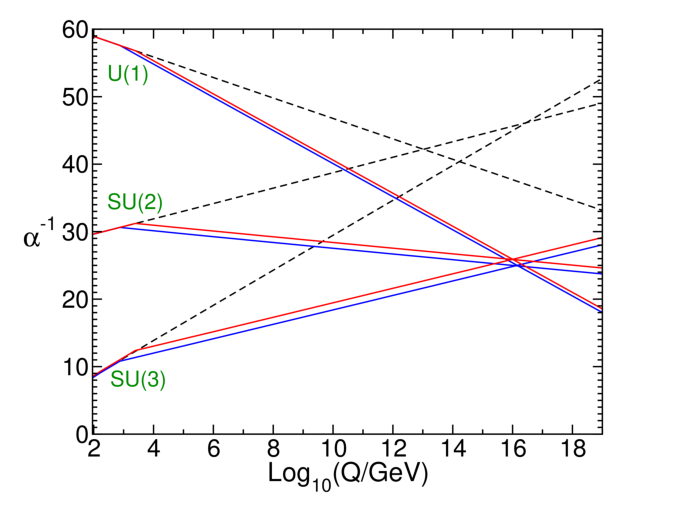
\includegraphics{running_susy.pdf}
  \caption{Force des couplages dans le Modèle Standard (ligne
    pointillée) et dans le MSSM (lignes pleines) en fonction de
    l'échelle d'énergie ($Q$). Figure tirée de la
    réf.~\cite{martin_supersymmetry_1997}}
  \label{fig:unification}
\end{figure}

\section{Le Modèle Standard Minimalement Supersymmétrique}
\label{sec:susy:mssm}

% intro
En soit, la supersymétrie n'est pas une théorie mais bien un principe
général de symétrie entre bosons et fermions qui pourrait faire partie
d'une théorie sous-jacente au Modèle Standard. Puisque la
supersymétrie requiert la présence de nouvelles particules, il faut
trouver l'ensemble minimal de particules suplémmentaires qu'il faut
introduire au Modèle Standard pour avoir une théorie viable où le
lagrangien possède cette symérie. Puisque cette symétrie, si elle
existe, est nécessairement brisée en dessous d'une échelle d'au moins
l'ordre du TeV mais que le mécanisme de brisure n'est pas connu, il
faut incorporer au modèle une paramétrisation de ce mécanisme. Il en
résulte un modèle appelé \emph{Modèle Standard Minimalement
  Supersymétrique}, ou MSSM. 

Au total, le MSSM compte 124 paramètres: 19 paramètres venant du
Modèle Standard et 105 nouveaux paramètres, la plupart étant les
masses des superpartenaires (elles ne sont pas prédites par la
théorie), des angles de mélange ainsi que des phases quantifiant la
violation CP additionelle introduite par le MSSM.

\subsection{Les superparticules du MSSM}
\label{sec:susy:mssm:sparticules}

\subsubsection{Superpartenaires des fermions}

Les fermions du Modèle Standard ont un spin de $\frac{1}{2}$. Il
existe donc pour chaque fermion deux états propres de chiralité, droit
($R$) et gauche ($L$), qui correspondent à la projection du spin dans
la direction du mouvement dans la limite $E \gg m$. Il existe donc
deux superpartenaires pour chaque fermions, un par état de chiralité,
sauf pour les neutrinos qui n'ont qu'un état $L$~\cite{thomson_modern_2013}.

Ces \emph{sfermions} ne sont pas nécessairement des états propres de
masses, et les états physiques observables peuvent être des
combinaison linéaires des constituants de la paire associé à chaque
fermion. Dans la plupart des modèles le mélange entre les
superpartenaires des deux premières générations de quarks sont
négligeables et on peut les dénoter par la chiralité de leur
partenaire du MS. Le mélange entre les sfermions de la troisième
génération ne peut en général pas être
négligé~\cite{aad_summary_2015}.

La troisième génération de squark revêt un intérêt particulier
lorsqu'on considère le problème de la hiérarchie. En effet, ce sont
ces squarks qui, parmi les superpartenaires, occasionnent les
corrections à la masse du Higgs les plus
importantes~\cite{olive_susy2_2014}. Comme discuté dans la
section~\ref{sec:susy:th}, ces corrections sont proportionelles à la
masse des paraticules et ne doivent pas être trop élevés pour que le
problème de la hiérarchie soit réglé dans le MSSM. Les masses des
squarks top et bottom doivent alors être de l'ordre du TeV et sont
donc activement recherchés au LHC (TODO cite Gtt paper).

\subsubsection{Superpartenaires des bosons}
%% gauginos
Comme vu en section~\ref{sec:ms:th:struct:ewk}, les bosons
électrofaibles observés sont des combinaisons linéaires des bosons du
Modèle Standard $W^{(1)}, W^{(2)}, W^{(3)} et B$. De façon analogue,
les superpartenaires électrofaibles, les \emph{gauginos} sont associés
à ces états fondamentaux et les états observés sont de façon générale
être des combinaisons linéaires. Le mélange n'est cependant pas prédit
par la théorie et entre dans le modèle comme un ensemble de
paramètres~\cite{olive_susy1_2014}. Il y a deux types de gauginos:
ceux résultant du mélange de gauginos électriquement chargés, les
quatres \emph{chaginos}, notés $\chi_{1,2}^\pm$ ainsi que ceux
résultant du mélange des gauginos neutres, les quatres
\emph{neutralinos}, notés $\chi_{1,2,3,4}^0$\footnote{Les indices sont
  ordonné selon la masse de l'état, en ordre
  croissant.}\cite{aad_summary_2015}.

%% higgsinos
Le MSSM contient plusieurs partenaires du Higgs, les
\emph{Higgsino}. Il y en a 5 au total (2 chargés, 3 neutres). C'est le
nombre minimal qu'il faut introduire dans la théorie pour éviter
l'apparition d'anomalies~\cite{olive_susy1_2014}.

%% gluinos
Le MSSM est complété par le \emph{gluino}, le superpartenaire du gluon
du Modèle Standard. Le gluino peut potentiellement apporter des
corrections importantes aux masses des squark top, et donc sa masse
doit aussi être de l'ordre du TeV pour que le problème de la
hiérarchie soit réglé dans le MSSM (TODO cite Gtt paper).

\subsection{La R-parité}
\label{sec:susy:R}

La force des couplages ne conservant pas les nombres baryoniques~($B$)
et leptoniques~($L$) dans les théorie au-delà du Modèle Standard est
fortement contrainte par les mesure de la stabilité du proton. En
effet, si $B$ et $L$ ne sont pas conservés, le proton pourrait par
exemple se désintégrer en un positron et un pion neutre. Pour
accomoder la présente limite inférieure mesurée du temps de vie du
proton de $2.1 \times 10^{29}$
ans~\cite{kamland_collaboration_search_2006}, il est nécessaire que de
tels couplages soient très faibles.  Dans le Modèle Standard, cette
conservation n'est pas un principe fondamental mais bien une
conséquence de la structure du modèle: il n'y existe tout simplement
pas de termes possible violant la conservation de $B$ et $L$ qui soient
renormalisables. Or, il est possible d'inclure des intéractions
violant la conservation de $B$ et $L$ dans une extension
supersymmétrique du MS. Pour que la théorie soit viable, il faut donc
que ces couplages soit très faibles ou même nuls, ce qui motive
l'inclusion d'un principe de symétrie sous-jacent à la la
conservation de $B$ et $L$ dans le MSSM: la
\emph{R-parité}~\cite{martin_supersymmetry_1997}.

Chaque particules fondamentale se voit assigner une valeur de
$R$-parité, qui dépend de $B$, $L$ et du spin $S$ de la
particule:
\begin{eqnarray}
  R = (-1)^{3(B - L) + 2S}
\end{eqnarray}

Toutes les particules du Modèle Standard ont une $R$-parité de $+1$,
tandis que leurs superpartenaires ont tous une $R$-parité de $-1$. Ce
nombre est multiplicativement conservé dans toutes les intéractions du
MSSM, ce qui implique que tous les sommets d'intéractions ont un
nombre pair de particules supersymétriques. Ceci a de grandes
conséquences phénoménologiques: les particules supersymmétriques sont
toujours produites en nombre pairs lors de collisions de particules du
MS, et toutes particule supersymmétrique doit éventuellement se
désintégrer en états finaux contentant un nombre impair de particules
supersymmétriques. Cette dernière implication est très importante:
cela signifie que la particule supersymmétrique la plus légère est
stable~\cite{martin_supersymmetry_1997}. Cette particule est
différente selon la valeur des paramètres du modèles et est donc notée
$LSP$~\footnote{De l'anglais, \emph{Lightest Supersymmetric
    Particle}}. Si la LSP est le neutralino le plus léger, le
$\chi_1^0$, alors elle peut être un élément constituant la matière
sombre observée dans l'univers puisqu'elle a toute les caractéristique
d'une WIMP~\cite{olive_review_2014}.

% \subsection{Les paramètres du MSSM}
% \label{sec:susy:mssm:params}

% \subsection{Problèmes du MSSM}
% %* Problèmes avec le MSSM
% %% Pas une théorie complète (breaking?)
% %% Conserve pas nb leptonique
% %% trop de FCNC
% %% trop de violation CP
% %% c'est une bonne chose!

%%% Local Variables:
%%% mode: latex
%%% TeX-master: "memoire"
%%% End:
